% <- percent signs are used to comment
\documentclass[12pt]{article}

%%%%%% PACKAGES - this part loads additional material for LaTeX %%%%%%%%%
% Nearly anything you want can be done in LaTeX if you load the right package 
% (search ctan.org or google it if you are looking for something).  We will load
% here a few that we need for this document or that we expect you to need later.

% The next 3 lines are needed to fix shortcomings of TeX that only make sense given its 40-year history ...
% Simple keep and ignore.
\usepackage[utf8]{inputenc}
\usepackage[T1]{fontenc}
\usepackage{lmodern}
\usepackage{amsmath}
\usepackage{changepage}
\usepackage{lipsum}

% Custom margins (and paper sizes etc.) because LaTeX else wastes much space
\usepackage[margin=1in]{geometry}

% The following packages are created by the American Mathematical Society (AMS)
% and provide lots of tools for special fonts, symbols, theorems, and proof
\usepackage{amsmath,amsfonts,amssymb,amsthm}
% mathtools contains many detail improvements over ams and core tex
\usepackage{mathtools}

% graphicx is required for images
\usepackage{graphicx}

% enumitem used for customizing enumerations
\usepackage[shortlabels]{enumitem}

% tikz is the package used for drawing, in particular for drawing trees. You may also find simplified packages like tikz-qtree and forest useful
\usepackage{tikz}

% hyperref allows links, urls, and many other PDF tricks.  We load it here
%          in such a way that the PDF file has info about it
\usepackage[%
	pdftitle={CS240 Assignment 0},%
	hidelinks,%
]{hyperref}


%%%%%% COMMANDS - here you can define your own LaTeX-commands %%%%%%%%%

%%%%%% End of Preamble %%%%%%%%%%%%%

\begin{document}

\begin{center}
{\Large\textbf{CS240, Spring 2022}}\\
\vspace{2mm}
{\Large\textbf{Assignment 3: Question 1}}\\
\vspace{3mm}
\end{center}
\begin{adjustwidth}{0em}{0pt}
\textbf{Q3b)} 
\begin{figure}[tbhp]
	\begin{center}
		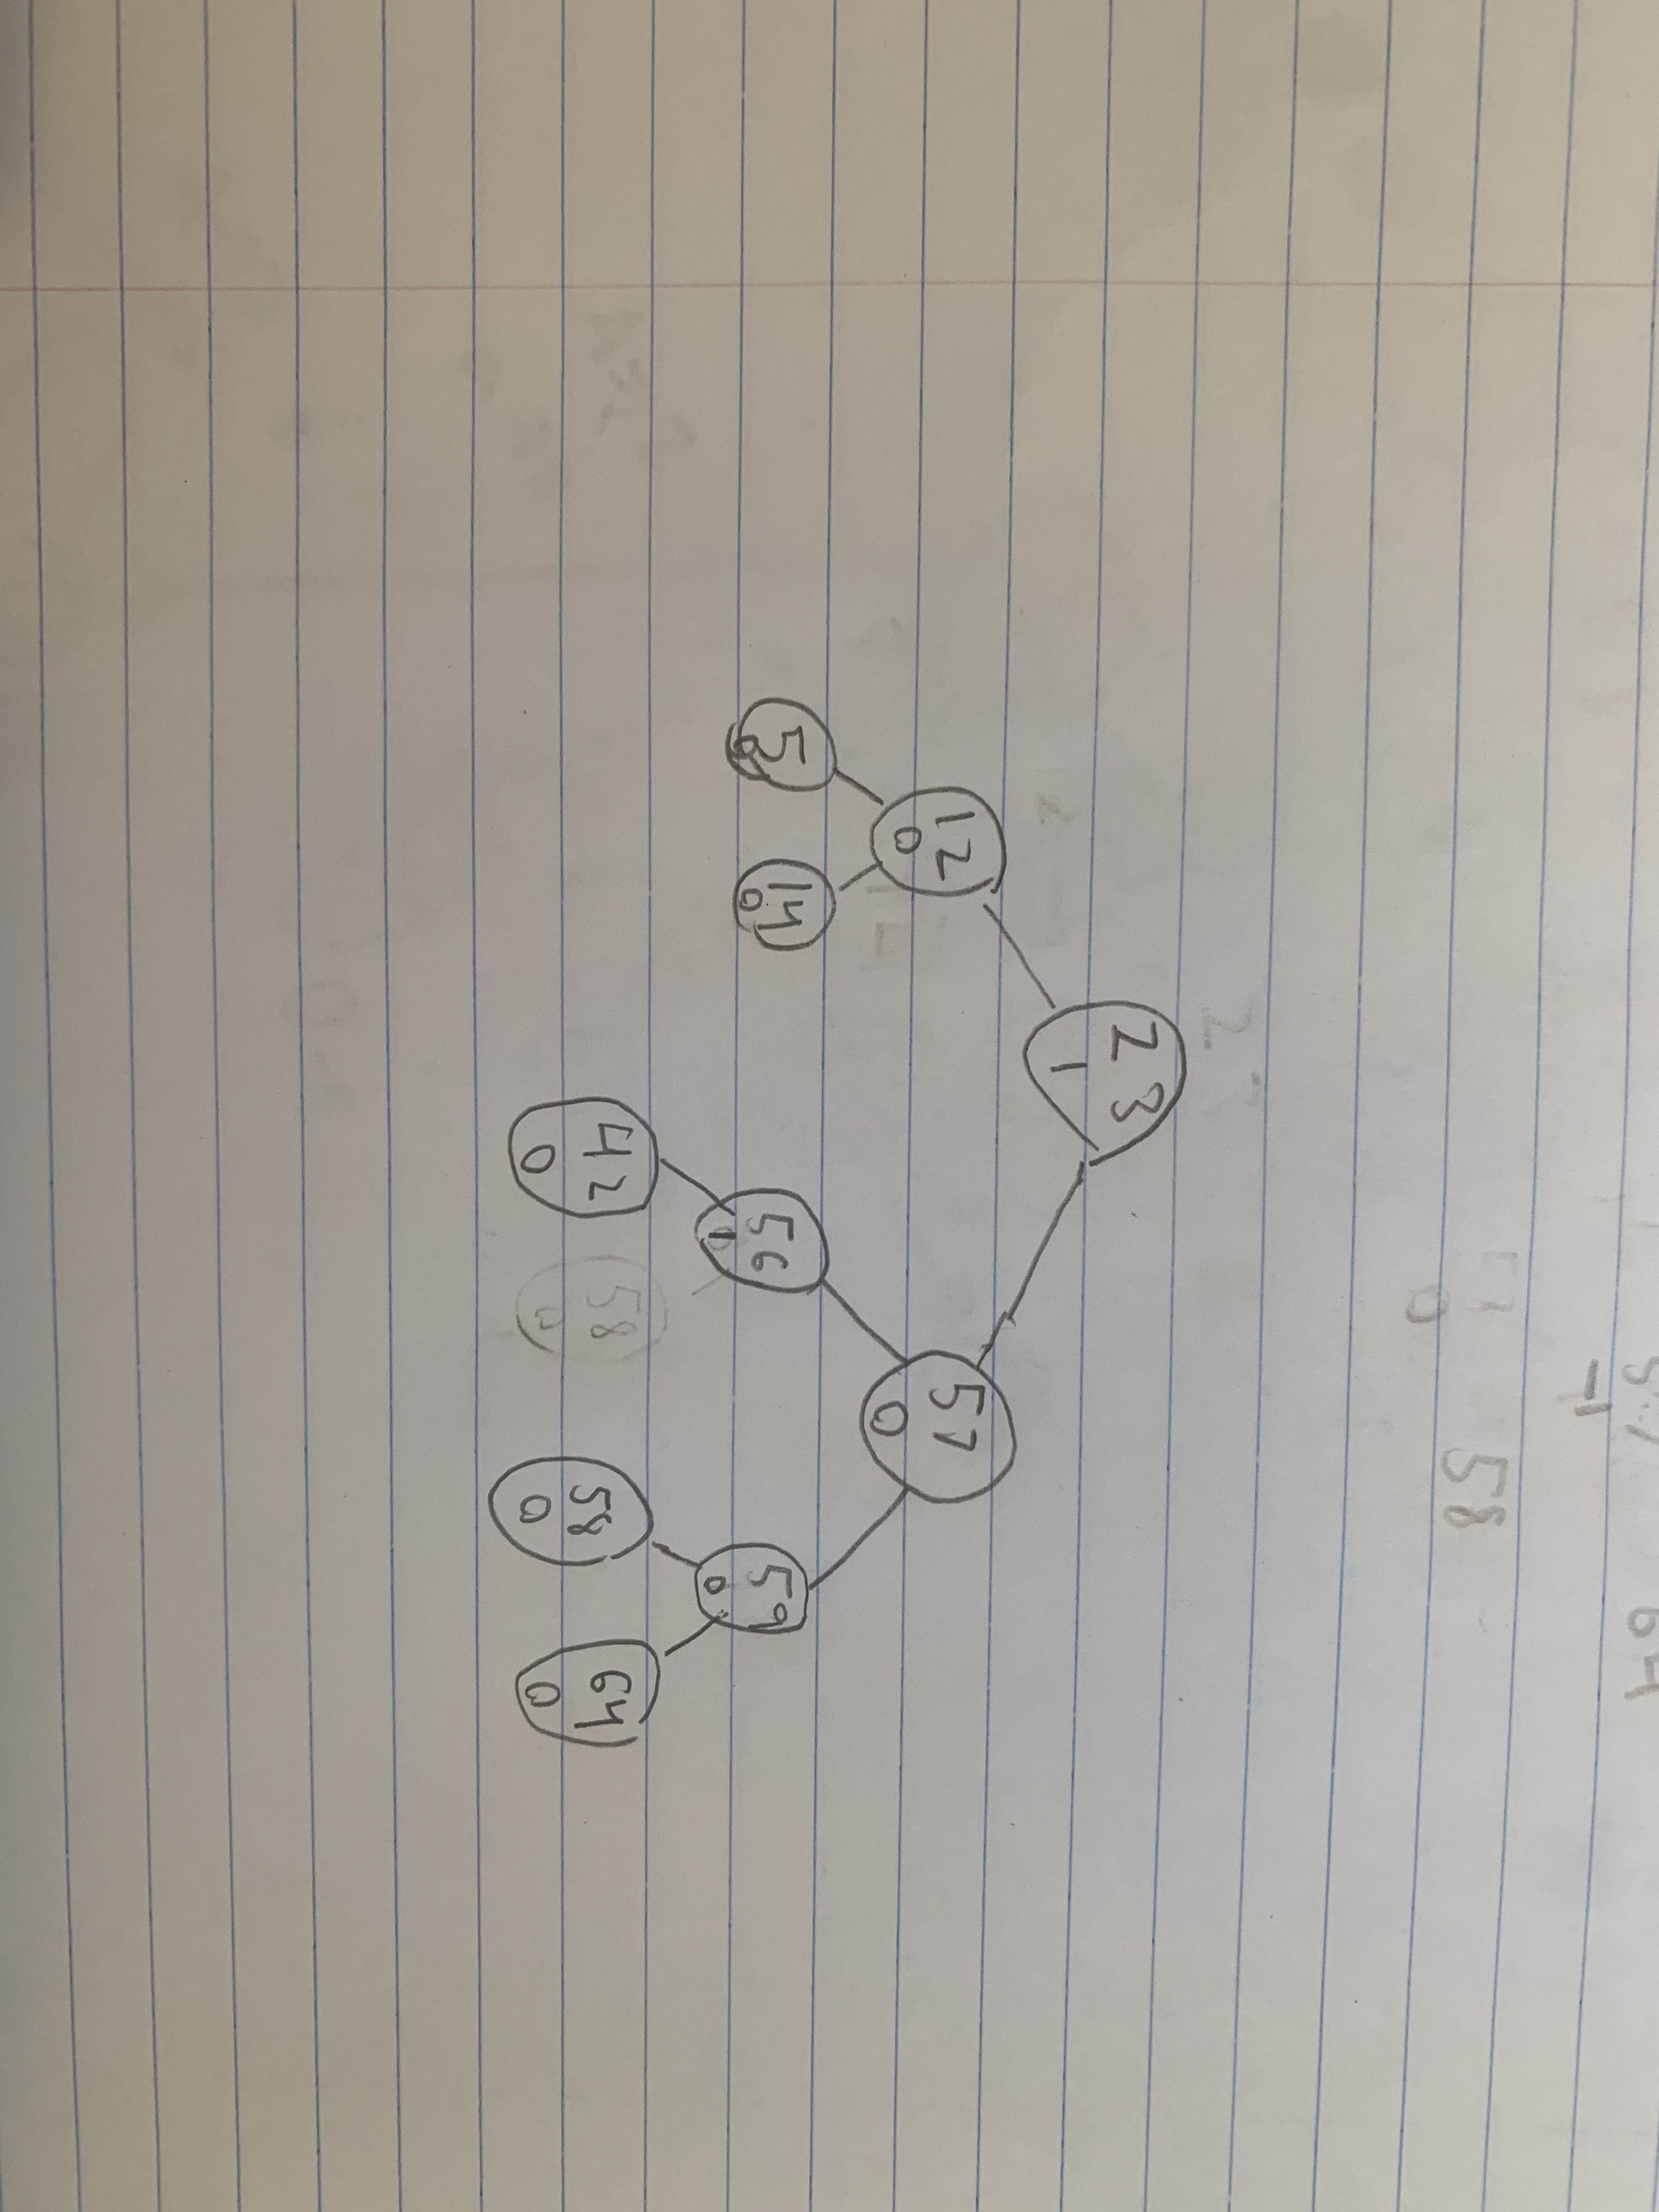
\includegraphics[width=0.4\textwidth, angle=90]{1st.jpg}
	\end{center}
	\caption{AVL tree after 58 is inserted}
	\label{figcaption}
	\begin{center}
		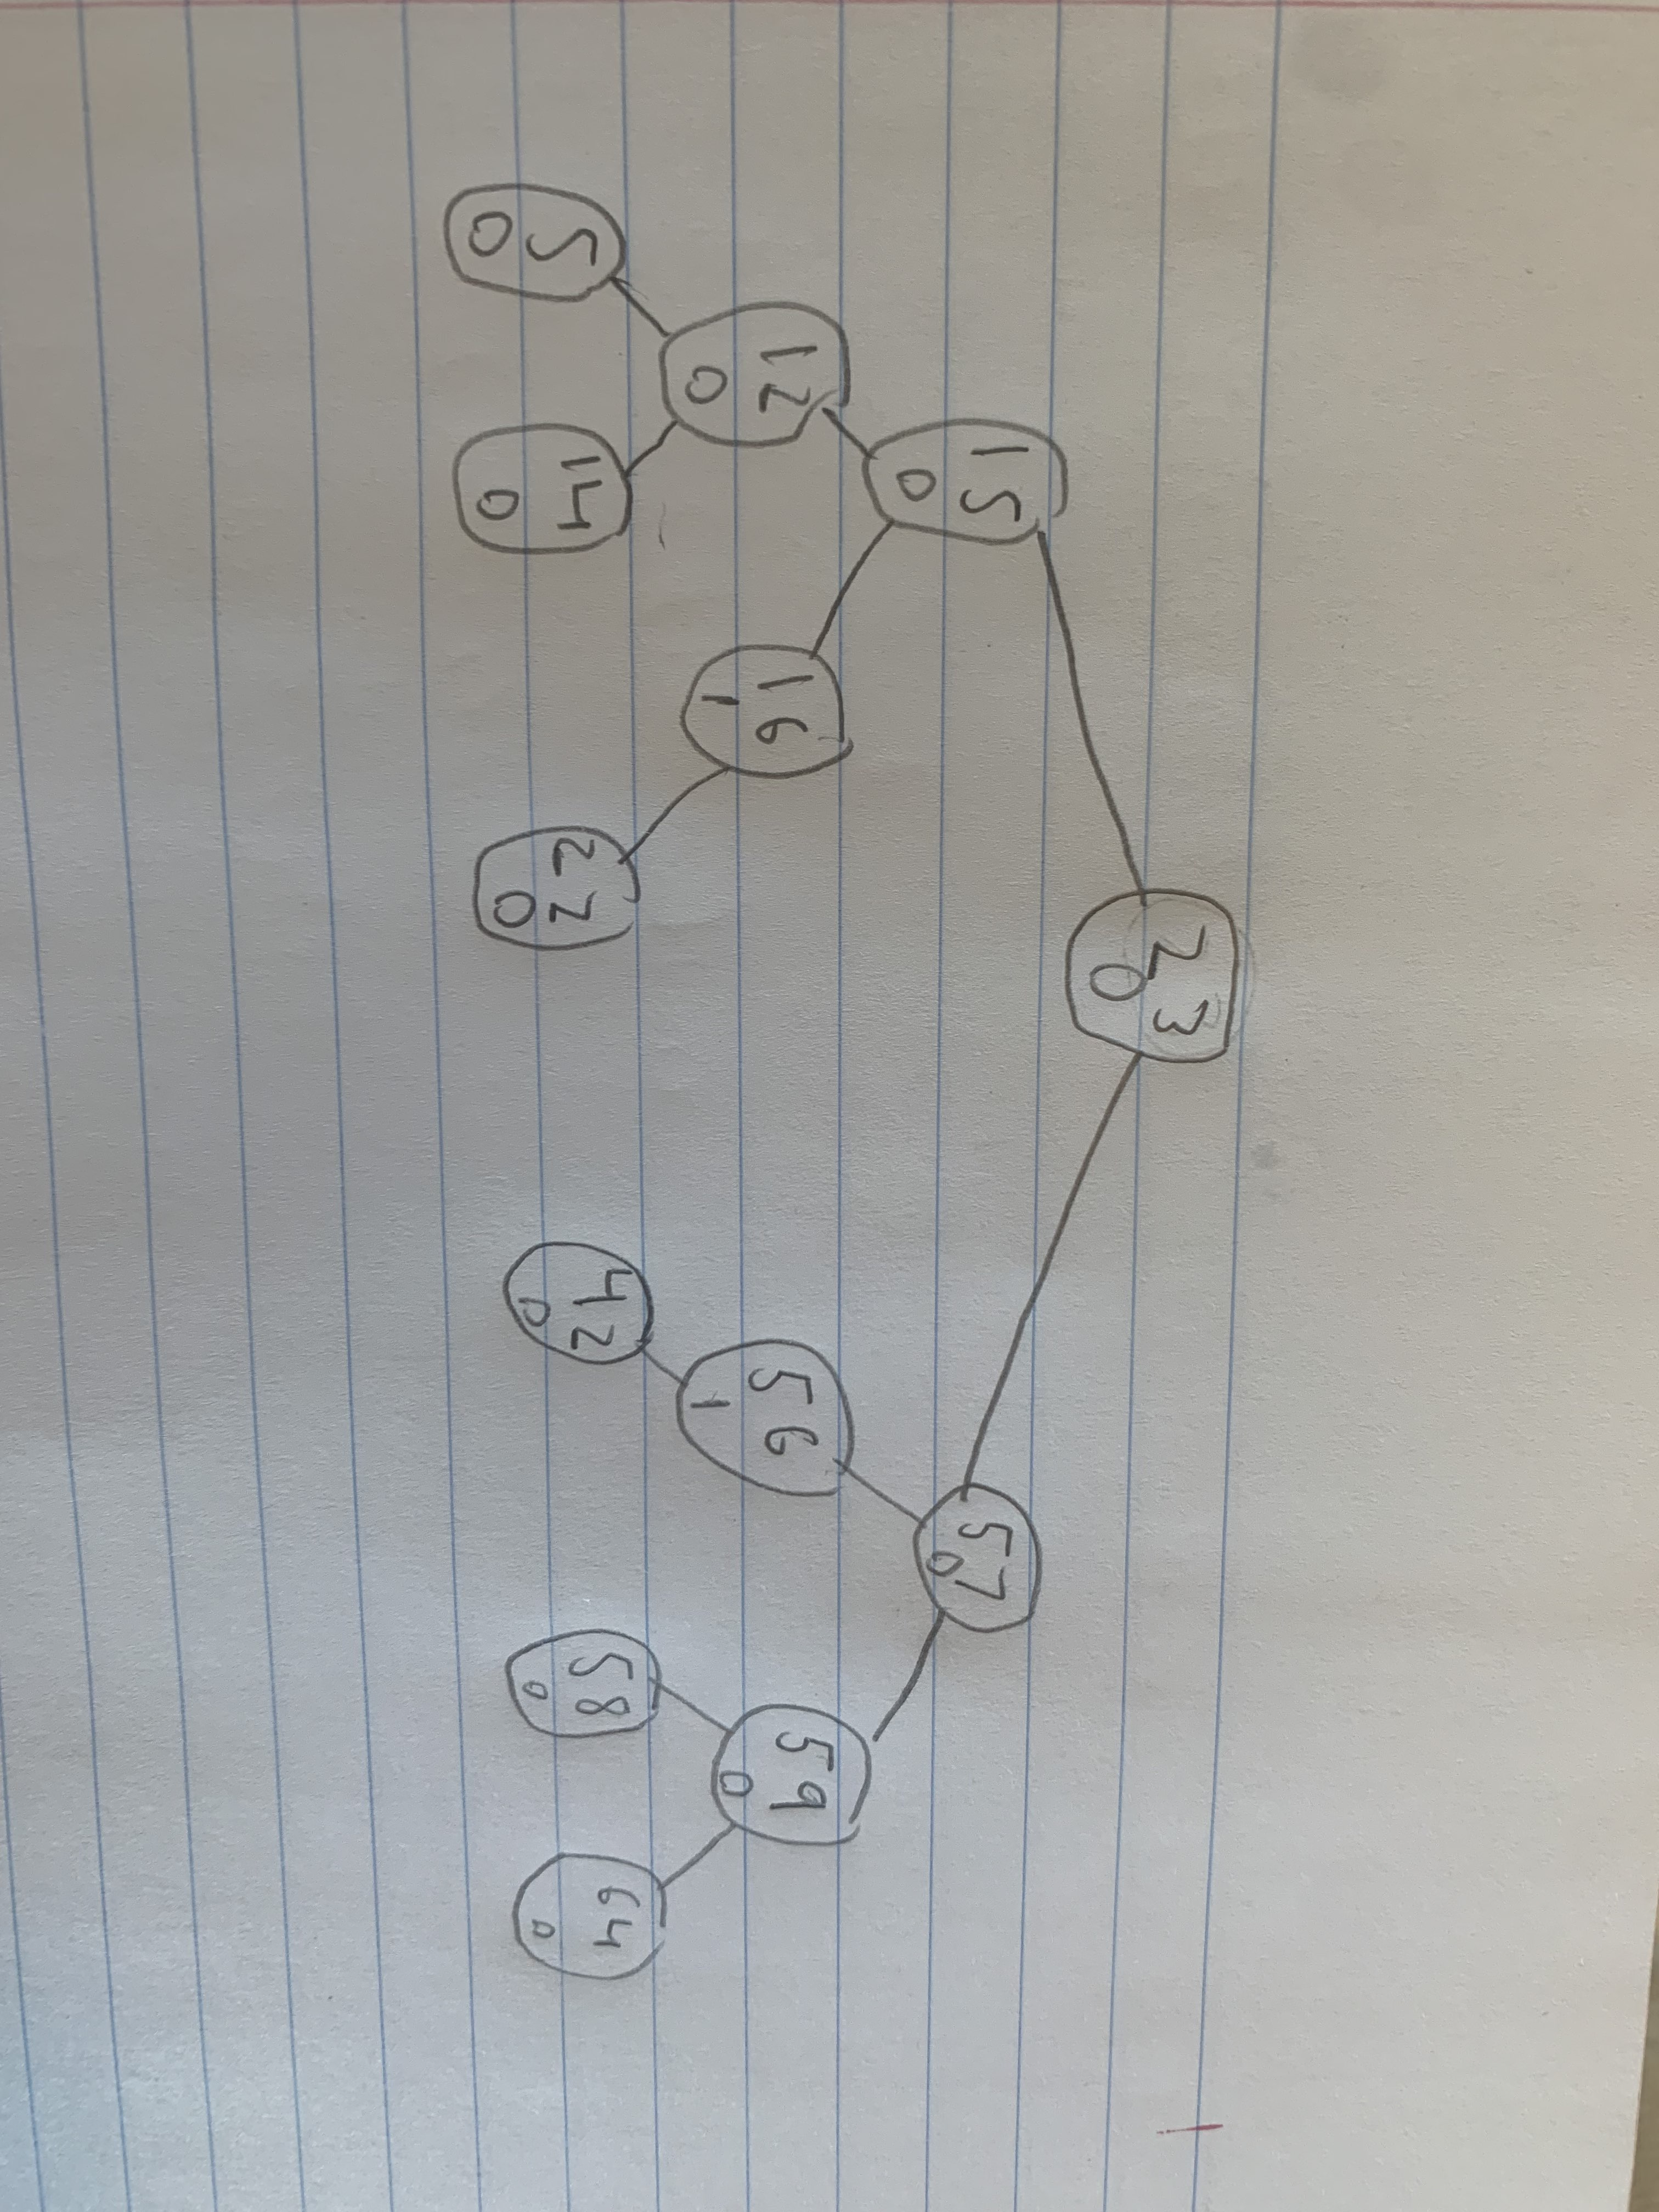
\includegraphics[width=0.4\textwidth, angle=90]{2nd.jpg}
	\end{center}
	\caption{AVL tree after 22 is inserted}
	\label{figcaption}
\end{figure}
\end{adjustwidth} 
\newpage
\begin{adjustwidth}{0em}{0pt}
\textbf{Q3c)}
In order to derive this we would first make an array of all the nodes in the AVL tree and we would sort this array.
\[ [5, 12, 14, 15, 16, 22, 23, 42, 56, 57, 58, 59, 64] \]
From this array we would pick the middle element (using the floor) and then split the array into two around the element we would removed, this would give us:
\[ \text{inserted = } [23] \]
\[ [5, 12, 14, 15, 16, 22], [42, 56, 57, 58, 59, 64] \]
Repeating the process for both arrays (working left to right our next step would give us:
\[ \text{inserted = } [23, 14, 57] \]
\[ [5, 12], [15, 16, 22], [42, 56], [58, 59, 64] \]
Repeating this again we get:
\[ \text{inserted = } [23, 14, 57, 5, 16, 42, 59] \]
\[12], [15], [22], [56], [58], [64] \]
Finally we would get that the order we should insert nodes in as:
\[ [23, 14, 57, 5, 16, 42, 59, 12, 15, 22, 56, 58, 64] \]
In general we would create a recursive algorithm which given an array would print the middle element (calculated using the floor), if the array is only size 1 we would stop otherwise we would split the array into half around the middle element and run the algorithm on it
\end{adjustwidth} 
\newpage
\textbf{Q3d)} 
\begin{figure}[tbhp]
	\begin{center}
		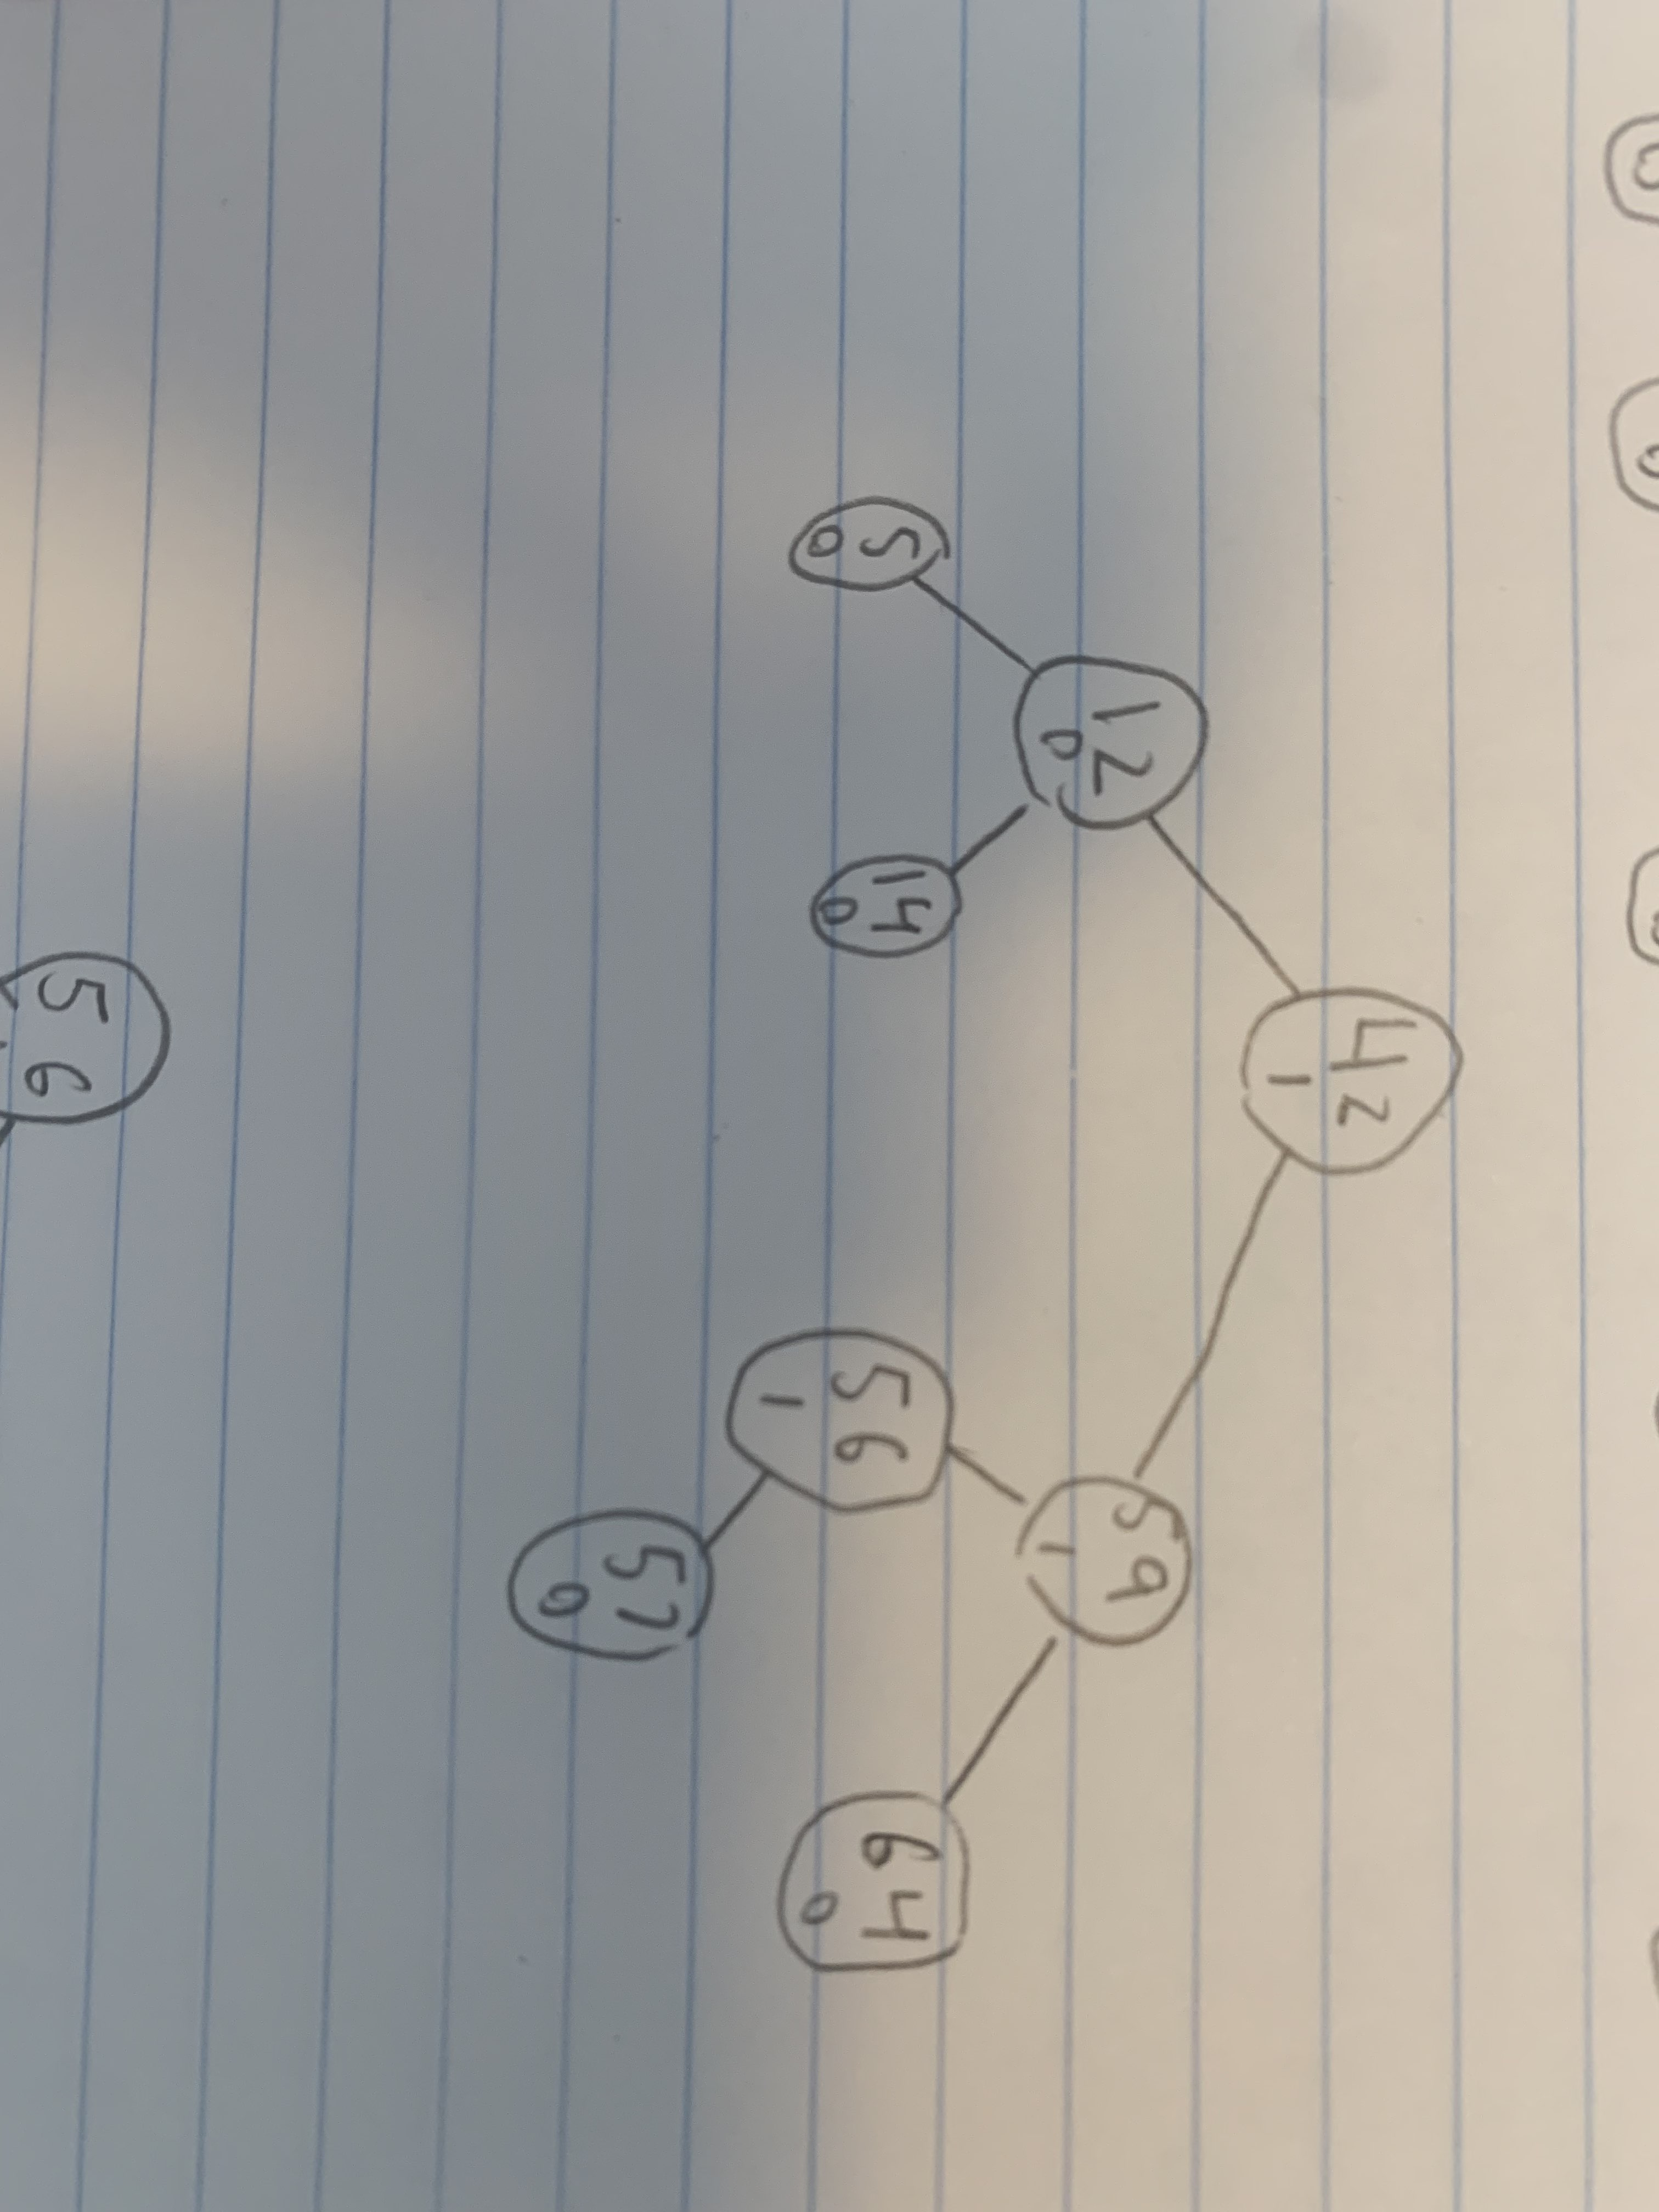
\includegraphics[width=0.4\textwidth, angle=90]{3.jpg}
	\end{center}
	\caption{AVL tree after 23 is deleted}
	\label{figcaption}
	\begin{center}
		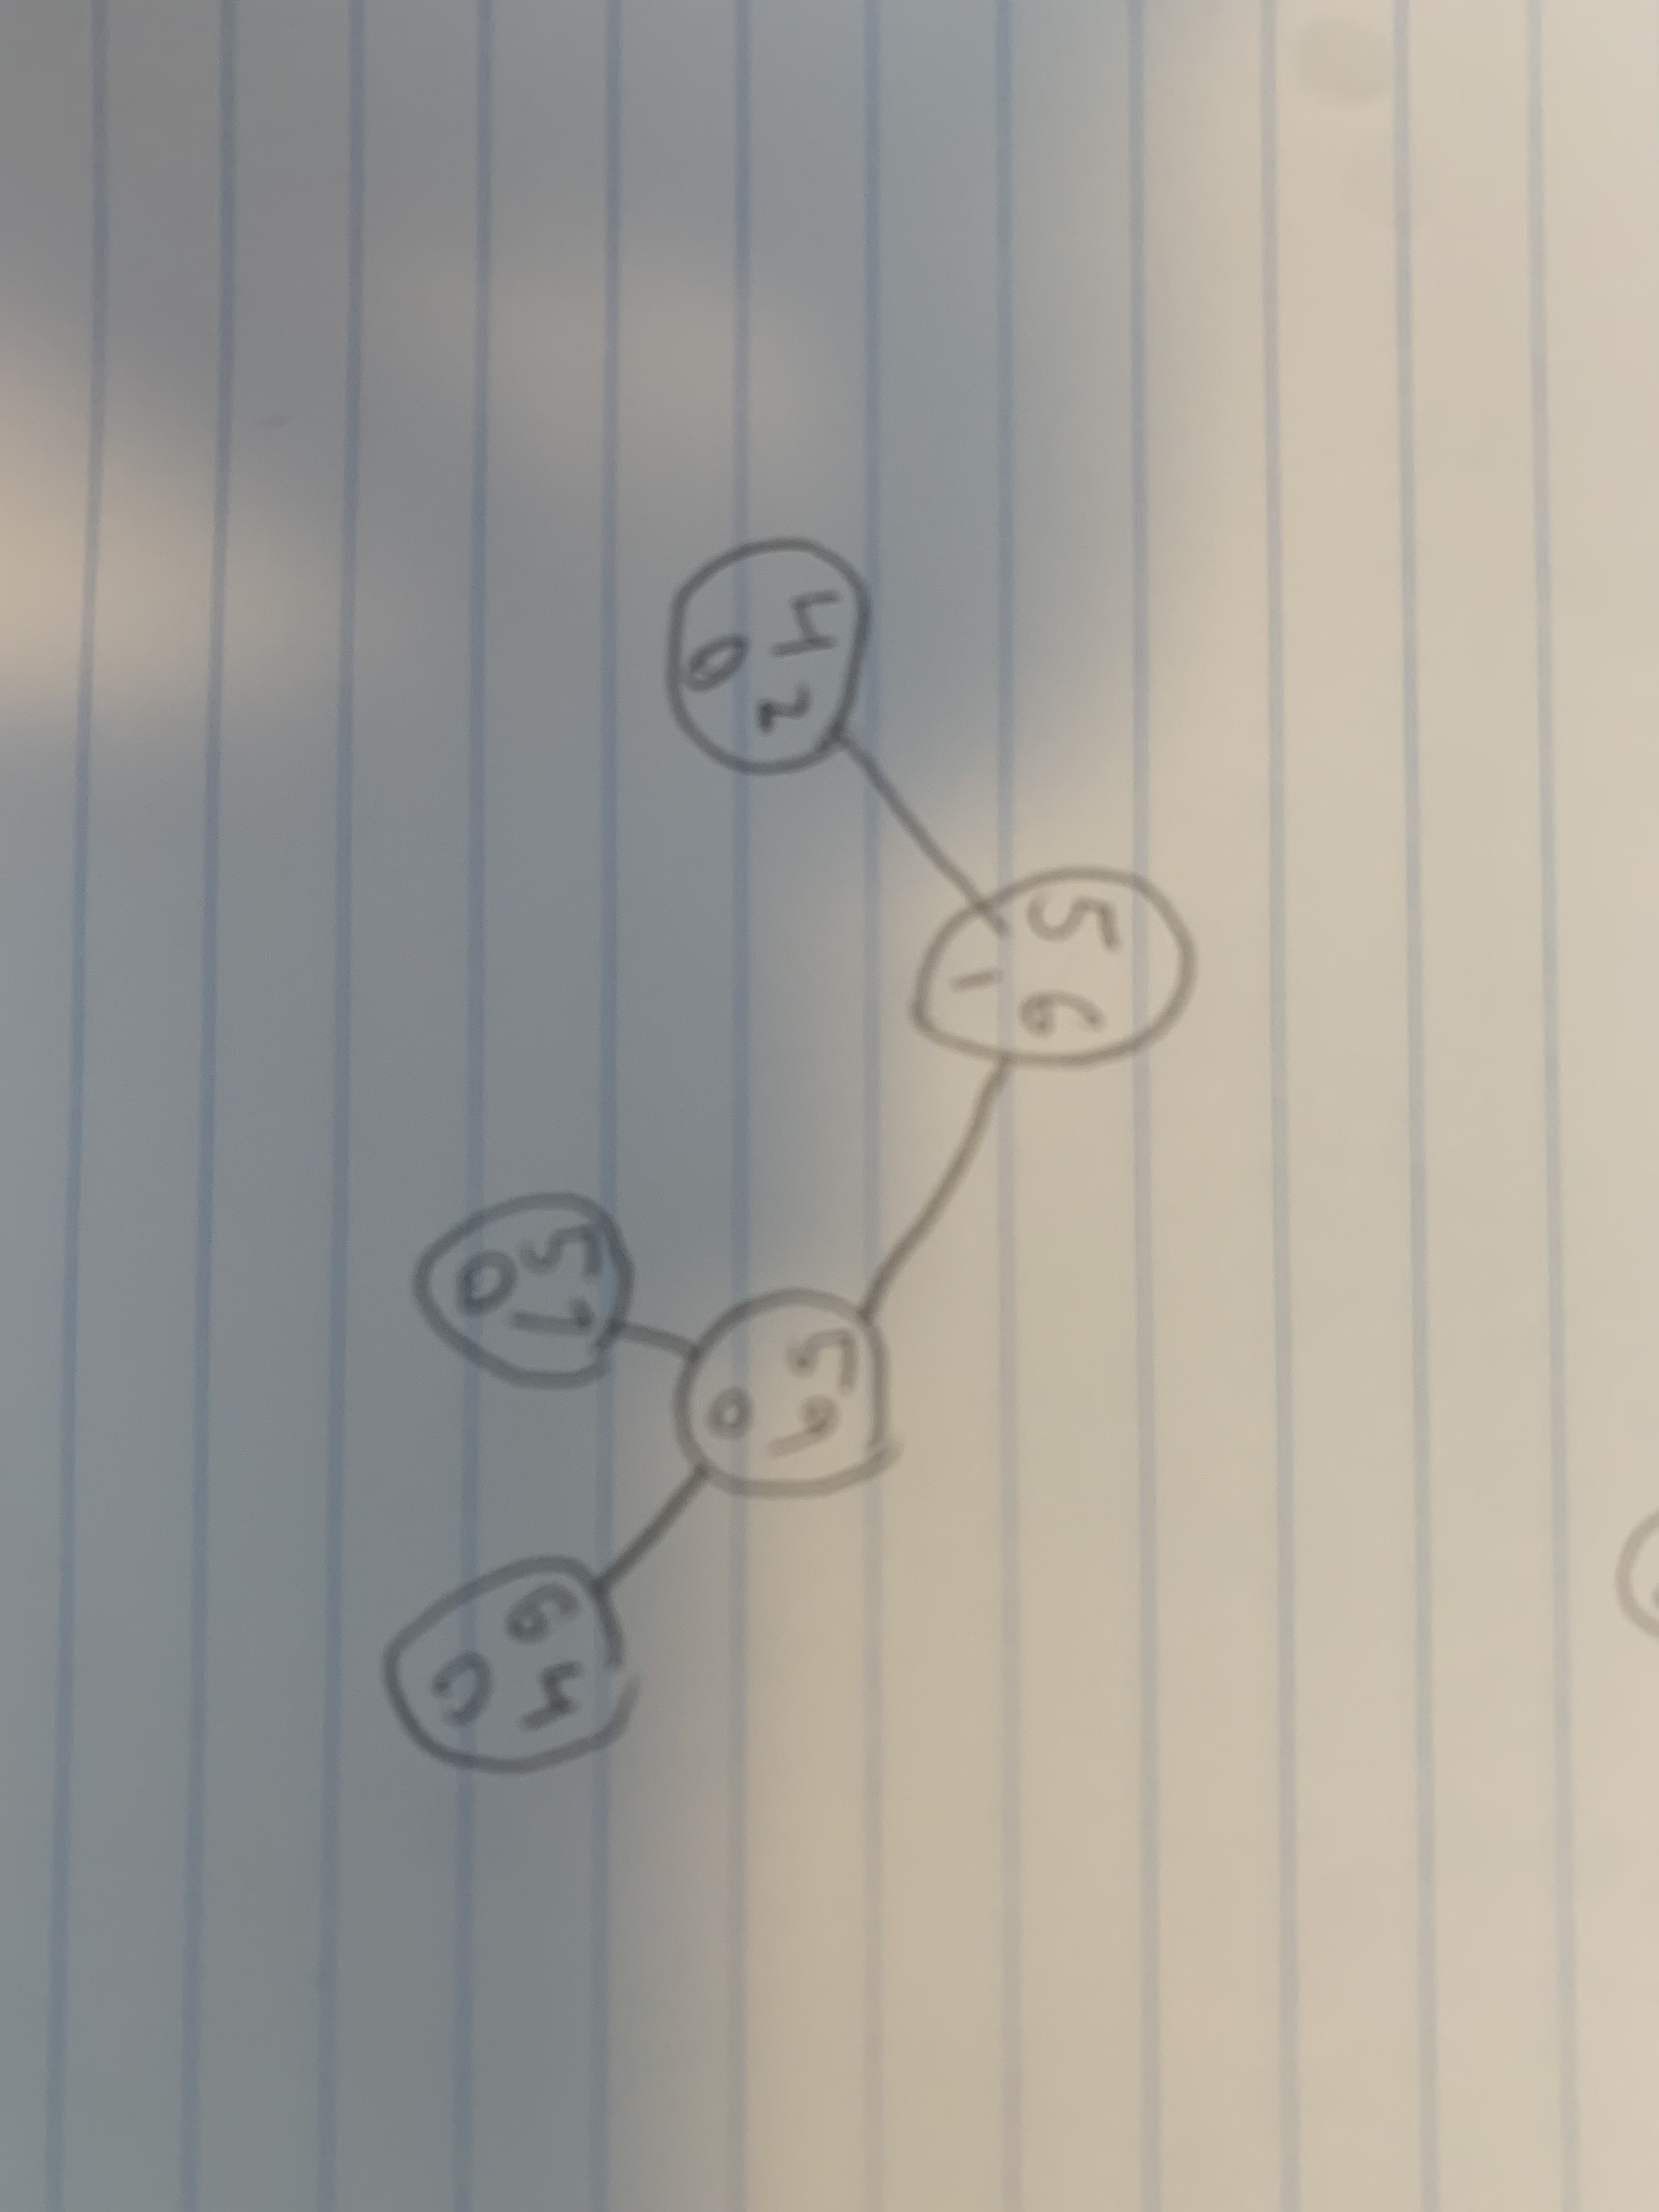
\includegraphics[width=0.4\textwidth, angle=90]{4.jpg}
	\end{center}
	\caption{AVL tree after 5 is deleted}
	\label{figcaption}
\end{figure}



\end{document}